\subsection{Software Privilege Levels}
\label{sec:rings}

In an Infrastructure-as-a-Service (IaaS) cloud environment, such as Amazon EC2,
commodity CPUs run software at four different privilege levels. The rest of the
section describes the privilege levels. We also point to successful exploits
that execute at each privilege level, motivating the SGX design decision to
assume that the host computer has malicious software running at all privilege
levels.

Figure~\ref{fig:cpu_rings} shows the privilege levels in the Intel
architecture. Software running at each level is strictly more powerful than
software running at less privileged levels. It follows that software running at
a level can access the code and data at less privileged levels, and compromise
the software running at these levels. Thus, software at each level must trust
all the software running at more privileged levels.

\begin{figure}[hbtp]
  \center{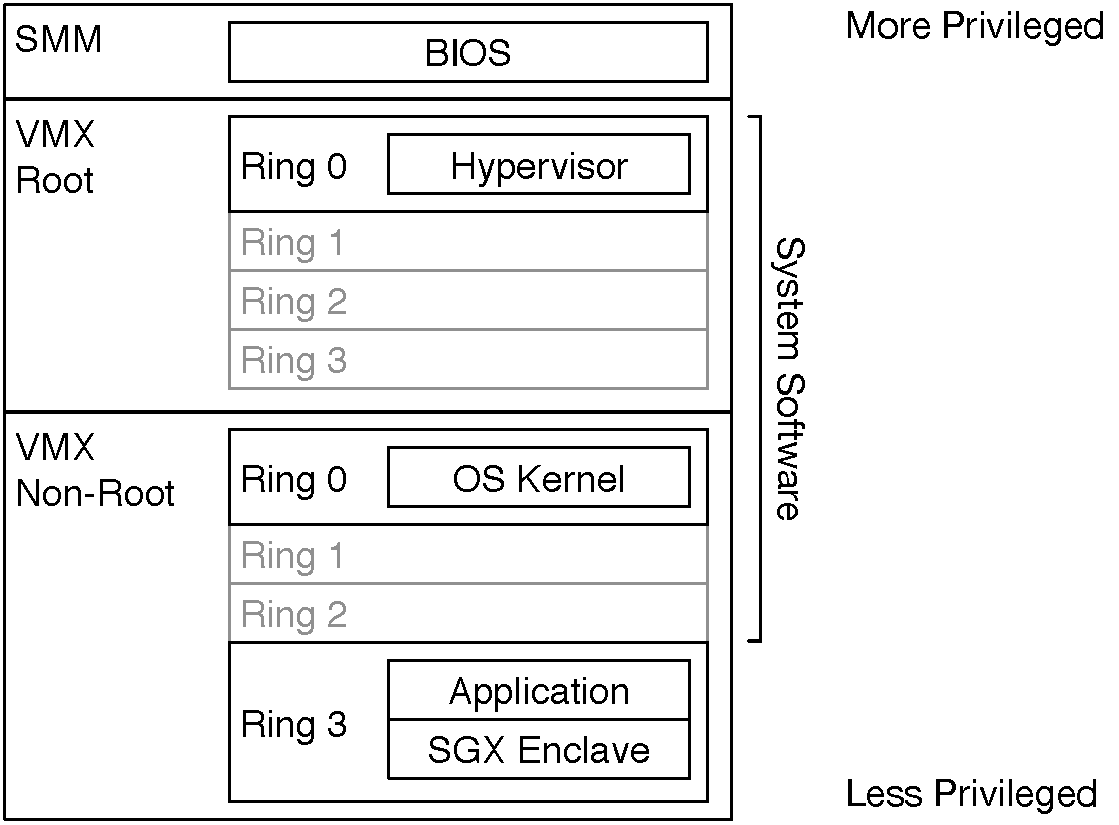
\includegraphics[width=85mm]{figures/cpu_rings.pdf}}
  \caption{
    The privilege levels in the x86 architecture, and the software that
    typically runs at each security level.
  }
  \label{fig:cpu_rings}
\end{figure}

% System Management Mode: SDM S 34

\textit{System Management Mode} (SMM) is intended for use by the motherboard
manufacturers to implement features such as fan control and deep sleep, and/or
to emulate missing hardware. SMM mode is entered by sending the CPU an SMI
signal, which was initially designed exclusively for hardware use, and only
produced when the SMI\# pin was asserted on the CPU's chip package. However, in
modern systems, system software can generate an SMI, using the methods in
\S~\ref{sec:interrupts}. This opens up the avenue for SMM-based software
exploits.

The SMM code and data are stored in a contiguous subset of DRAM called
\textit{System Management RAM} (SMRAM) which, in theory, is not readable or
writable when the processor isn't running in SMM. However, its protection
mechanisms were bypassed multiple times~\cite{duflot2006smm,
rutkowska2008remap, wojtczuk2009smm}, and SMM-based
rootkits~\cite{wecherowski2009smm, embleton2010smm} have been demonstrated.

IaaS cloud providers allow their customers to run their operating system of
choice in a virtualized environment. Hardware
virtualization~\cite{uhlig2005vmx}, called \textit{Virtual Machine Extensions}
(VMX) by Intel, adds support for a \textit{hypervisor}, also called a
Virtual Machine Monitor (VMM) in the Intel documentation. The hypervisor runs
at a higher privilege level (VMX root mode) than the operating system, and is
responsible for allocating hardware resources across multiple operating systems
that share the same physical machine. The hypervisor uses the CPU's hardware
virtualization features to make each operating system believe it is running in
its own computer, called a \textit{virtual machine} (VM). Hypervisor code
generally runs at ring 0 in VMX root mode.

The popular Xen hypervisor uses VMX root mode to obtain better peformance and a
smaller codebase \cite{zhang2008xen} than virtualization software based on
binary translation \cite{rosenblum2005virtualization}. Despite its relatively
small codebase, Xen has had over 40 security vulnerabilities patched in
\textbf{each} of the last three years (2012-2014) \cite{cvedetails2014xen}.

\cite{mccune2010trustvisor} proposes using a very small hypervisor together
with Intel TXT's dynamic root of trust for measurement (DRTM) to implement
trusted execution. \cite{vasudevan2010requirements} argues that a dynamic root
of trust mechanism, like Intel TXT, is necessary to ensure a hypervisor's
integrity.  Unfortunately, the TXT design requires an implementation complex
enough that security vulnerabilities have been found \cite{wojtczuk2009txt2}
\cite{wojtczuk2011txt}. Furthermore, any SMM attack can be used to compromise
TXT \cite{wojtczuk2009txt}.

The systems research literature recommends breaking up an operating system into
a small \textit{kernel}, which runs at a high privilege level, known as the
\textit{kernel mode} or \textit{supervisor mode} and, in the Intel
architecture, as \textit{ring 0}. The kernel allocates the computer's resources
to the other system components, such as device drivers and services, which run
at lower privilege levels. However, for performance reasons\footnote{Switching
between rings is much slower than a normal procedure call.}, mainstream
operating systems have large amounts of code running at ring 0. Their
\textit{monolithic kernels} include device drivers, filesystem code, networking
stacks, and video rendering functionality.

The monolithic kernel design leads to many opportunities for security
vulnerabilities in kernel code. For example the Linux kernel has had over 100
security vulnerabilities patched in \textbf{each} of the last three years
(2012-2014) \cite{cvedetails2014linux} \cite{chen2011linux}. Also, a successful
attack on SMM or the hypervisor trivially translates into a compromised kernel.

Application code, such as a Web server or a game client, runs at the lowest
privilege level, referred to as \textit{user mode} (\textit{ring 3} in the
Intel architecture). In IaaS cloud environments, the virtual machine images
provided by customers run in VMX non-root mode, so the kernel runs in VMX
non-root ring 0, and the application code runs in VMX non-root ring 3.
